% =====================================================================
% Supplementary Information (reconstructed editable LaTeX source).
% Built with tectonic: `tectonic supplement.tex`
% =====================================================================
\documentclass[11pt]{article}
\usepackage[margin=1in]{geometry}
\usepackage{graphicx}
\usepackage{amsmath}
\usepackage{amssymb}
\usepackage{microtype}
\usepackage{setspace}
\usepackage[font=small,labelfont=bf]{caption}
\usepackage[hidelinks]{hyperref}

\graphicspath{{../figures/manuscript/}}

\newcommand{\Dstar}{\ensuremath{D^{*}}}

\setstretch{1.15}
\setlength{\parskip}{0.5em}
\setlength{\parindent}{0pt}

% Number supplementary figures as S1, S2, ...
\renewcommand{\thefigure}{S\arabic{figure}}

\begin{document}

\begin{center}
{\Large\bfseries Supplementary Information\par}
\vspace{0.6em}
{\itshape Calibration and Efficiency of Uncertainty Estimates in Intravoxel Incoherent Motion
Imaging\par}
\vspace{0.4em}
Avery Karlin, BA --- Columbia University (Applied Physics and Applied Mathematics) and
University of Colorado Boulder (Computer Science)
\end{center}

\vspace{1em}

\section*{Supplementary Methods}

\subsection*{S1. Architecture ablation (Masked Autoregressive Flow)}

To test whether the \Dstar{} pointwise overconfidence is specific to the neural spline flow,
the density estimator was replaced with a Masked Autoregressive Flow (5 MADE layers) while
holding the permutation-invariant embedding network, the BoxUniform prior, the
$\log_{10}$-SNR conditioning, and the training budget identical to the primary configuration.
The MAF was audited on the same dense CRLB benchmarking grid; for \Dstar{} across the SNR
10--100 grid, the claimed posterior SD and the achieved empirical SD (scatter of the
posterior mean across 50 noise realizations) were recorded and expressed as a ratio to the
CRLB floor. No out-of-distribution, acquisition-shift, or in-vivo evaluations were repeated
for the MAF.

\subsection*{S2. Dense-acquisition control}

To separate prior-reversion from the sparsity of the clinical acquisition, a second NPE was
trained and evaluated entirely on a dense 16-point b-scheme ($\{0, 10, 20, 30, 50, 75, 100,
150, 200, 300, 400, 500, 600, 700, 800, 1000\}$~s/mm$^2$) under the identical recipe to the
primary model (set representation, neural spline flow, 500,000-simulation budget, log-\Dstar{}
prior, matched seed). The dense model is in-distribution for its own scheme (not the
off-scheme evaluation of Figure 4C) and is audited against the correspondingly tighter dense
CRLB floor; it trained to convergence (169 epochs). Per-SNR median \Dstar{} SD-to-CRLB ratios
reproduce the main-text Figure 3 transform over the 512-point grid.

\subsection*{S3. Operationalized out-of-distribution gate}

The deployment-time gate was operationalized at the voxel level on the in-vivo brain dataset
(OSIPI TF2.4 IVIM-MRI Code Collection data, Zenodo doi:10.5281/zenodo.14605039;
$N \approx 2{,}000$ gray-matter voxels). This is the same gray-matter ROI and held-out-b
partition as the $N = 500$ held-out-b coverage check in main-text Figure 4B; the larger sample
is drawn here because a per-voxel ROC threshold requires more voxels than an aggregate coverage
curve, and the two are overlapping random draws from the same voxel pool rather than distinct
datasets. For each voxel two deployable scores were computed
from the fit b-values only: the reduced $\chi^2$ of the biexponential NLLS fit (a classical,
NPE-independent goodness-of-fit signal) and an NPE posterior-predictive self-consistency
residual. Each was scored against the held-out-b posterior-predictive miscalibration
(computed on a disjoint b-value set, so prediction is a genuine generalization test, not a
tautology) by ROC AUC and by calibration recovery as a function of retained fraction. The
recommended threshold is the ROC Youden point of the self-consistency gate.

\subsection*{S5. Prior-sensitivity ablation}

To test whether the below-floor \Dstar{} overconfidence depends on the prior, a second NPE was
trained under the identical setB recipe (set representation, neural spline flow,
500,000-simulation budget, matched seed, clinical-sparse b-scheme), changing only the \Dstar{}
prior from log-uniform to a tissue-informed truncated Normal on $\log_{10}(\Dstar)$ ($\mu =
\log_{10}(0.03)$, $\sigma = 0.30$~dex). It was audited against the same analytical CRLB grid
and the same per-SNR median-ratio transform as the primary model.

\subsection*{S6. In-vivo cohort validation (liver)}

To test whether the in-vivo held-out-b overconfidence reproduces beyond a single subject, the
main-text held-out-b check was repeated across an open multi-subject liver IVIM dataset
(Dryad doi:10.5061/dryad.xwdbrv1cg; hypovascular liver lesions; GE Signa 1.5T; b-values
$\{0,10,25,50,200,500,800\}$~s/mm$^2$). This is an off-scheme deployment for the amortized NPE
(an independent vendor, field strength, organ, and b-scheme relative to the trained Philips 3T
clinical-sparse acquisition), i.e.\ the multi-subject analogue of the acquisition-shift result
(main-text Figure 4C). DICOM series were converted to NIfTI (\texttt{dcm2niix}); each b-value is
its own two-volume series carrying its own b=0, so each diffusion image was normalized by its
in-series b=0. Of 67 converted patients, 59 had all six non-zero b-series at a consistent
spatial geometry and were analyzed; the rest were excluded for missing or mismatched series.
Per patient, a fixed-seed random sample of foreground liver-parenchyma voxels (b=0 above a robust
threshold, finite and physically plausible attenuation across all b) was taken; the
normalized-signal noise level was estimated robustly as the median per-voxel biexponential
fit-residual RMS (giving SNR $\approx$ 13, typical for liver DWI at 1.5T), applied to both
estimators. Held-out-b posterior-predictive coverage was then computed exactly as in
\texttt{run\_f\_realdata.py} (fit on $b\in\{0,25,200,800\}$, held out $b\in\{10,50,500\}$),
comparing the amortized NPE to the per-voxel NLLS reference. Because in vivo lacks voxel-level
ground truth, this compares the two estimators rather than either against truth. The full
per-patient table and aggregates are released in the reproducibility module
(\texttt{npe/run\_liver\_cohort.py}).

\section*{Supplementary Figures}

\begin{figure}[htbp]
\centering
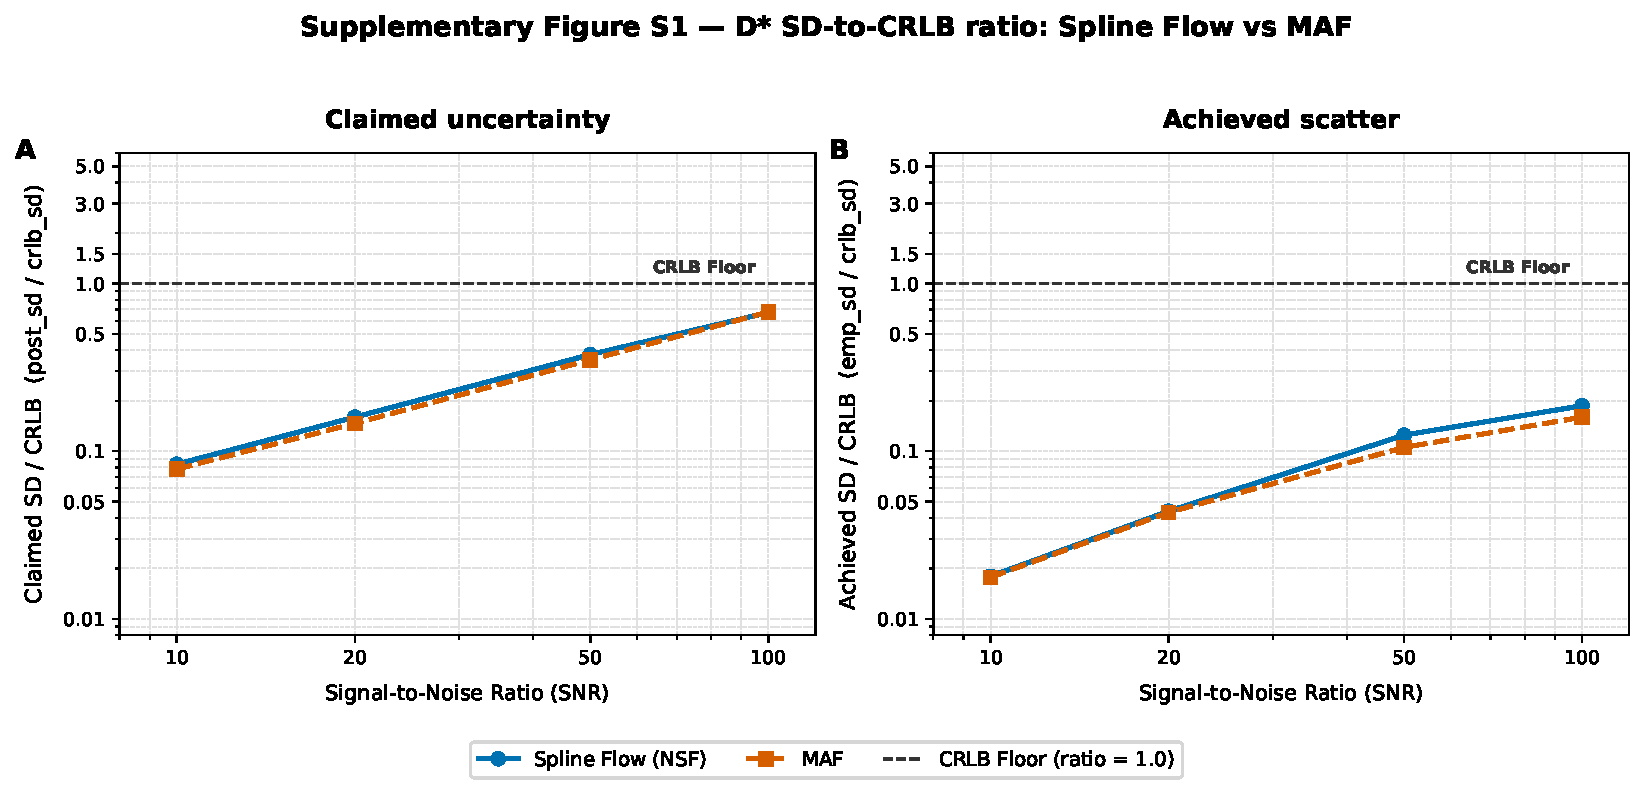
\includegraphics[width=\textwidth]{figS1_maf_ablation.pdf}
\caption{Architecture ablation. \Dstar{} SD-to-CRLB ratio versus SNR for the neural spline
flow and the Masked Autoregressive Flow (per-SNR medians). (A) Claimed posterior SD ratio;
(B) achieved empirical SD ratio. Both architectures sit well below the CRLB floor (ratio =
1.0) across SNR, with the MAF reproducing the same below-floor overconfidence (claimed ratio
within 6--8\% of the spline flow at SNR 10--50 and within 1\% at SNR 100; achieved ratio
within $\sim$15\% across SNR), indicating the \Dstar{} overconfidence is architecture-agnostic
rather than an artifact of the spline-flow density estimator.}
\end{figure}

\begin{figure}[htbp]
\centering
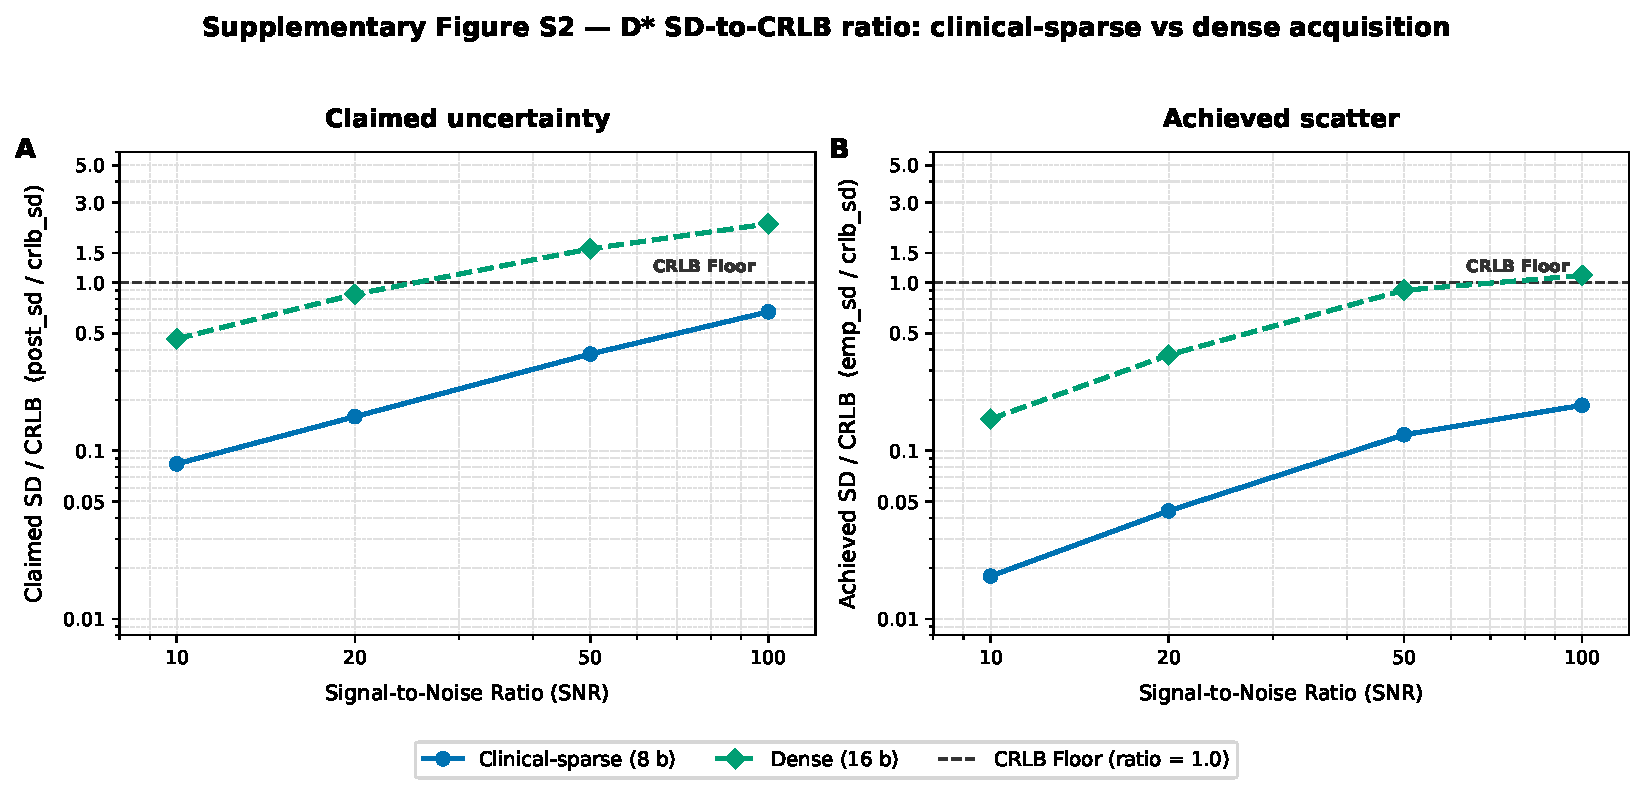
\includegraphics[width=\textwidth]{figS2_dense_acquisition.pdf}
\caption{Dense-acquisition control. \Dstar{} SD-to-CRLB ratio versus SNR for the
clinical-sparse (8 b) and dense (16 b) NPEs, each audited against its own CRLB floor. (A)
Claimed posterior SD ratio; (B) achieved empirical SD ratio. The dense model's claimed \Dstar{}
uncertainty stays below the floor through the clinical SNR regime (ratio 0.46 at SNR 10, 0.85
at SNR 20; 41\% of grid points overconfident overall vs 69\% clinical-sparse), crossing to
inefficiency only at high SNR. The below-floor overconfidence is mitigated but not eliminated
by denser sampling.}
\end{figure}

\begin{figure}[htbp]
\centering
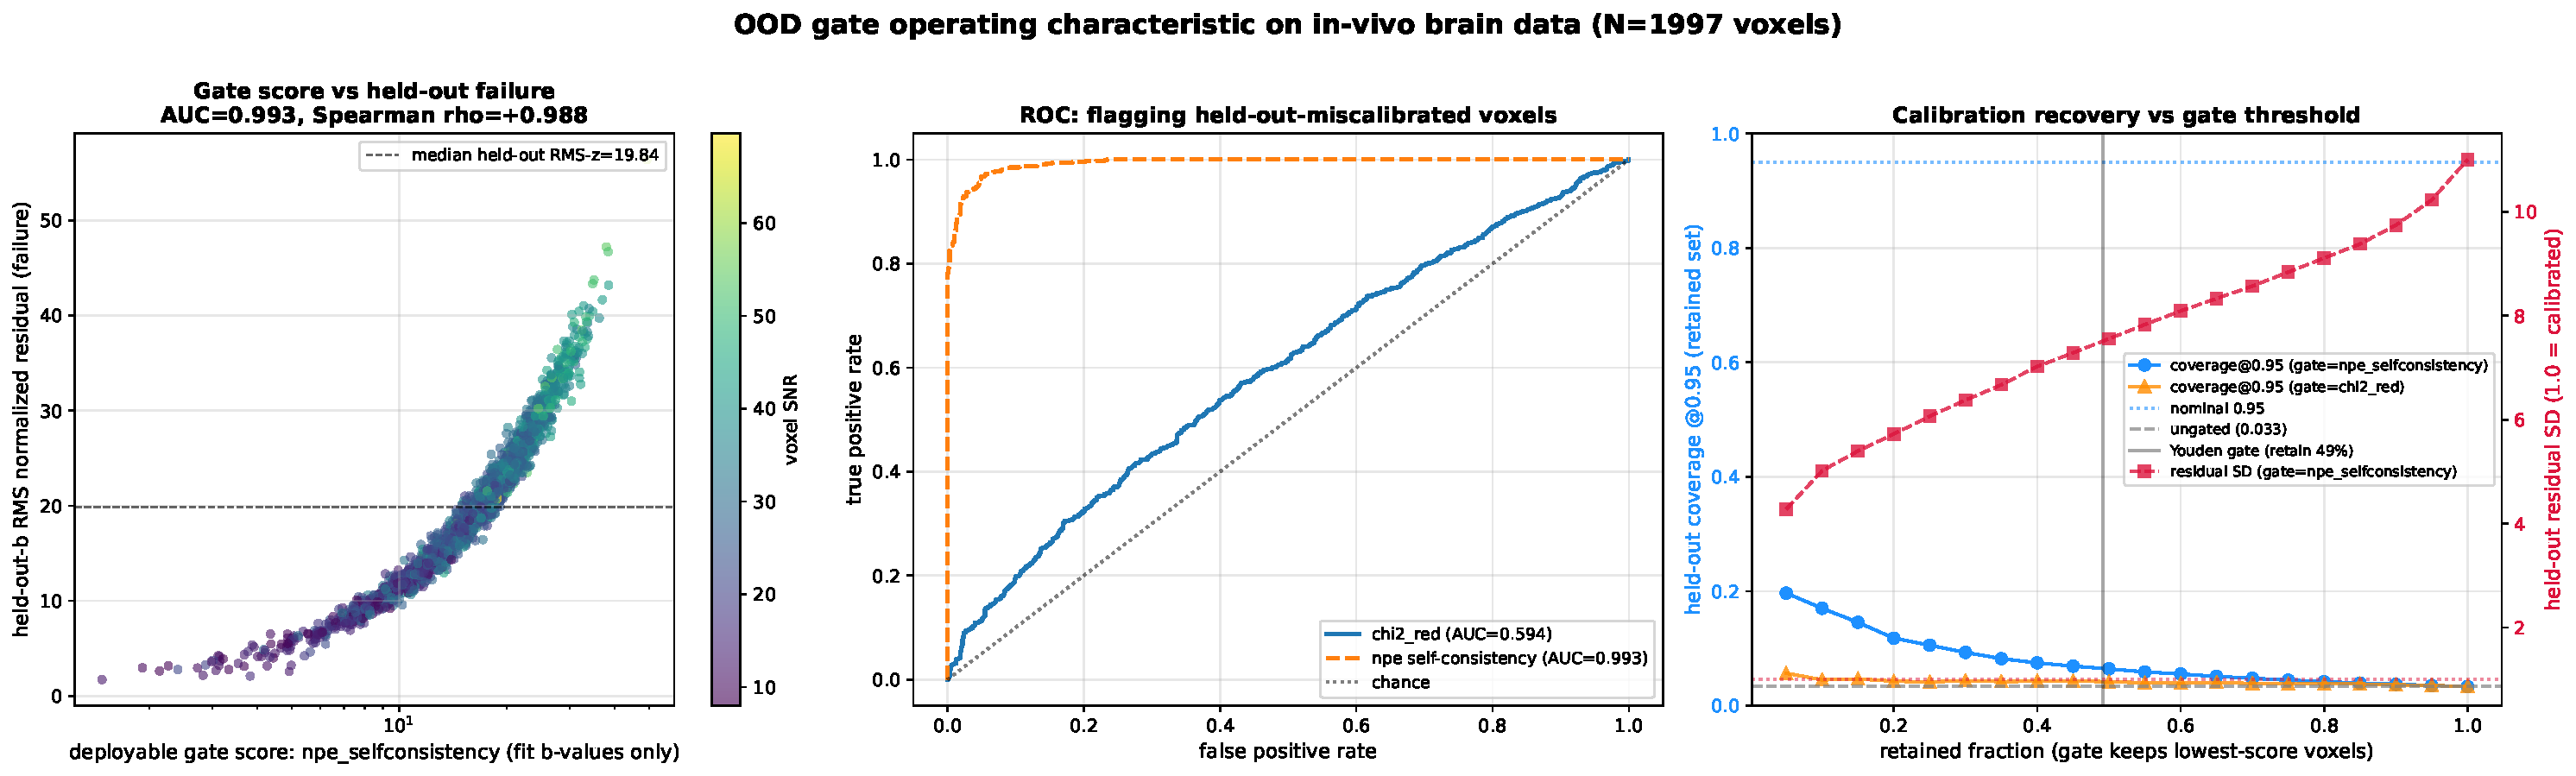
\includegraphics[width=\textwidth]{figS3_ood_gating.pdf}
\caption{Deployable out-of-distribution gate on the in-vivo brain dataset. (A) Held-out-b
coverage and (B) held-out normalized-residual SD as the retained voxel fraction is tightened,
for the NPE posterior-predictive self-consistency gate (AUC 0.99 against the unobservable
held-out miscalibration) versus a classical biexponential goodness-of-fit $\chi^2$ gate (AUC
0.59). The self-consistency gate monotonically recovers coverage ($0.03 \to 0.20$) and reduces
residual SD ($11.0 \to 4.3$); the $\chi^2$ gate does not, confirming the overconfidence is
intrinsic to the estimator rather than model-misfit. Marked point: ROC Youden threshold
(self-consistency $\le 16.7$, TPR 0.97 / FPR 0.05, 49\% retained).}
\end{figure}

\begin{figure}[htbp]
\centering
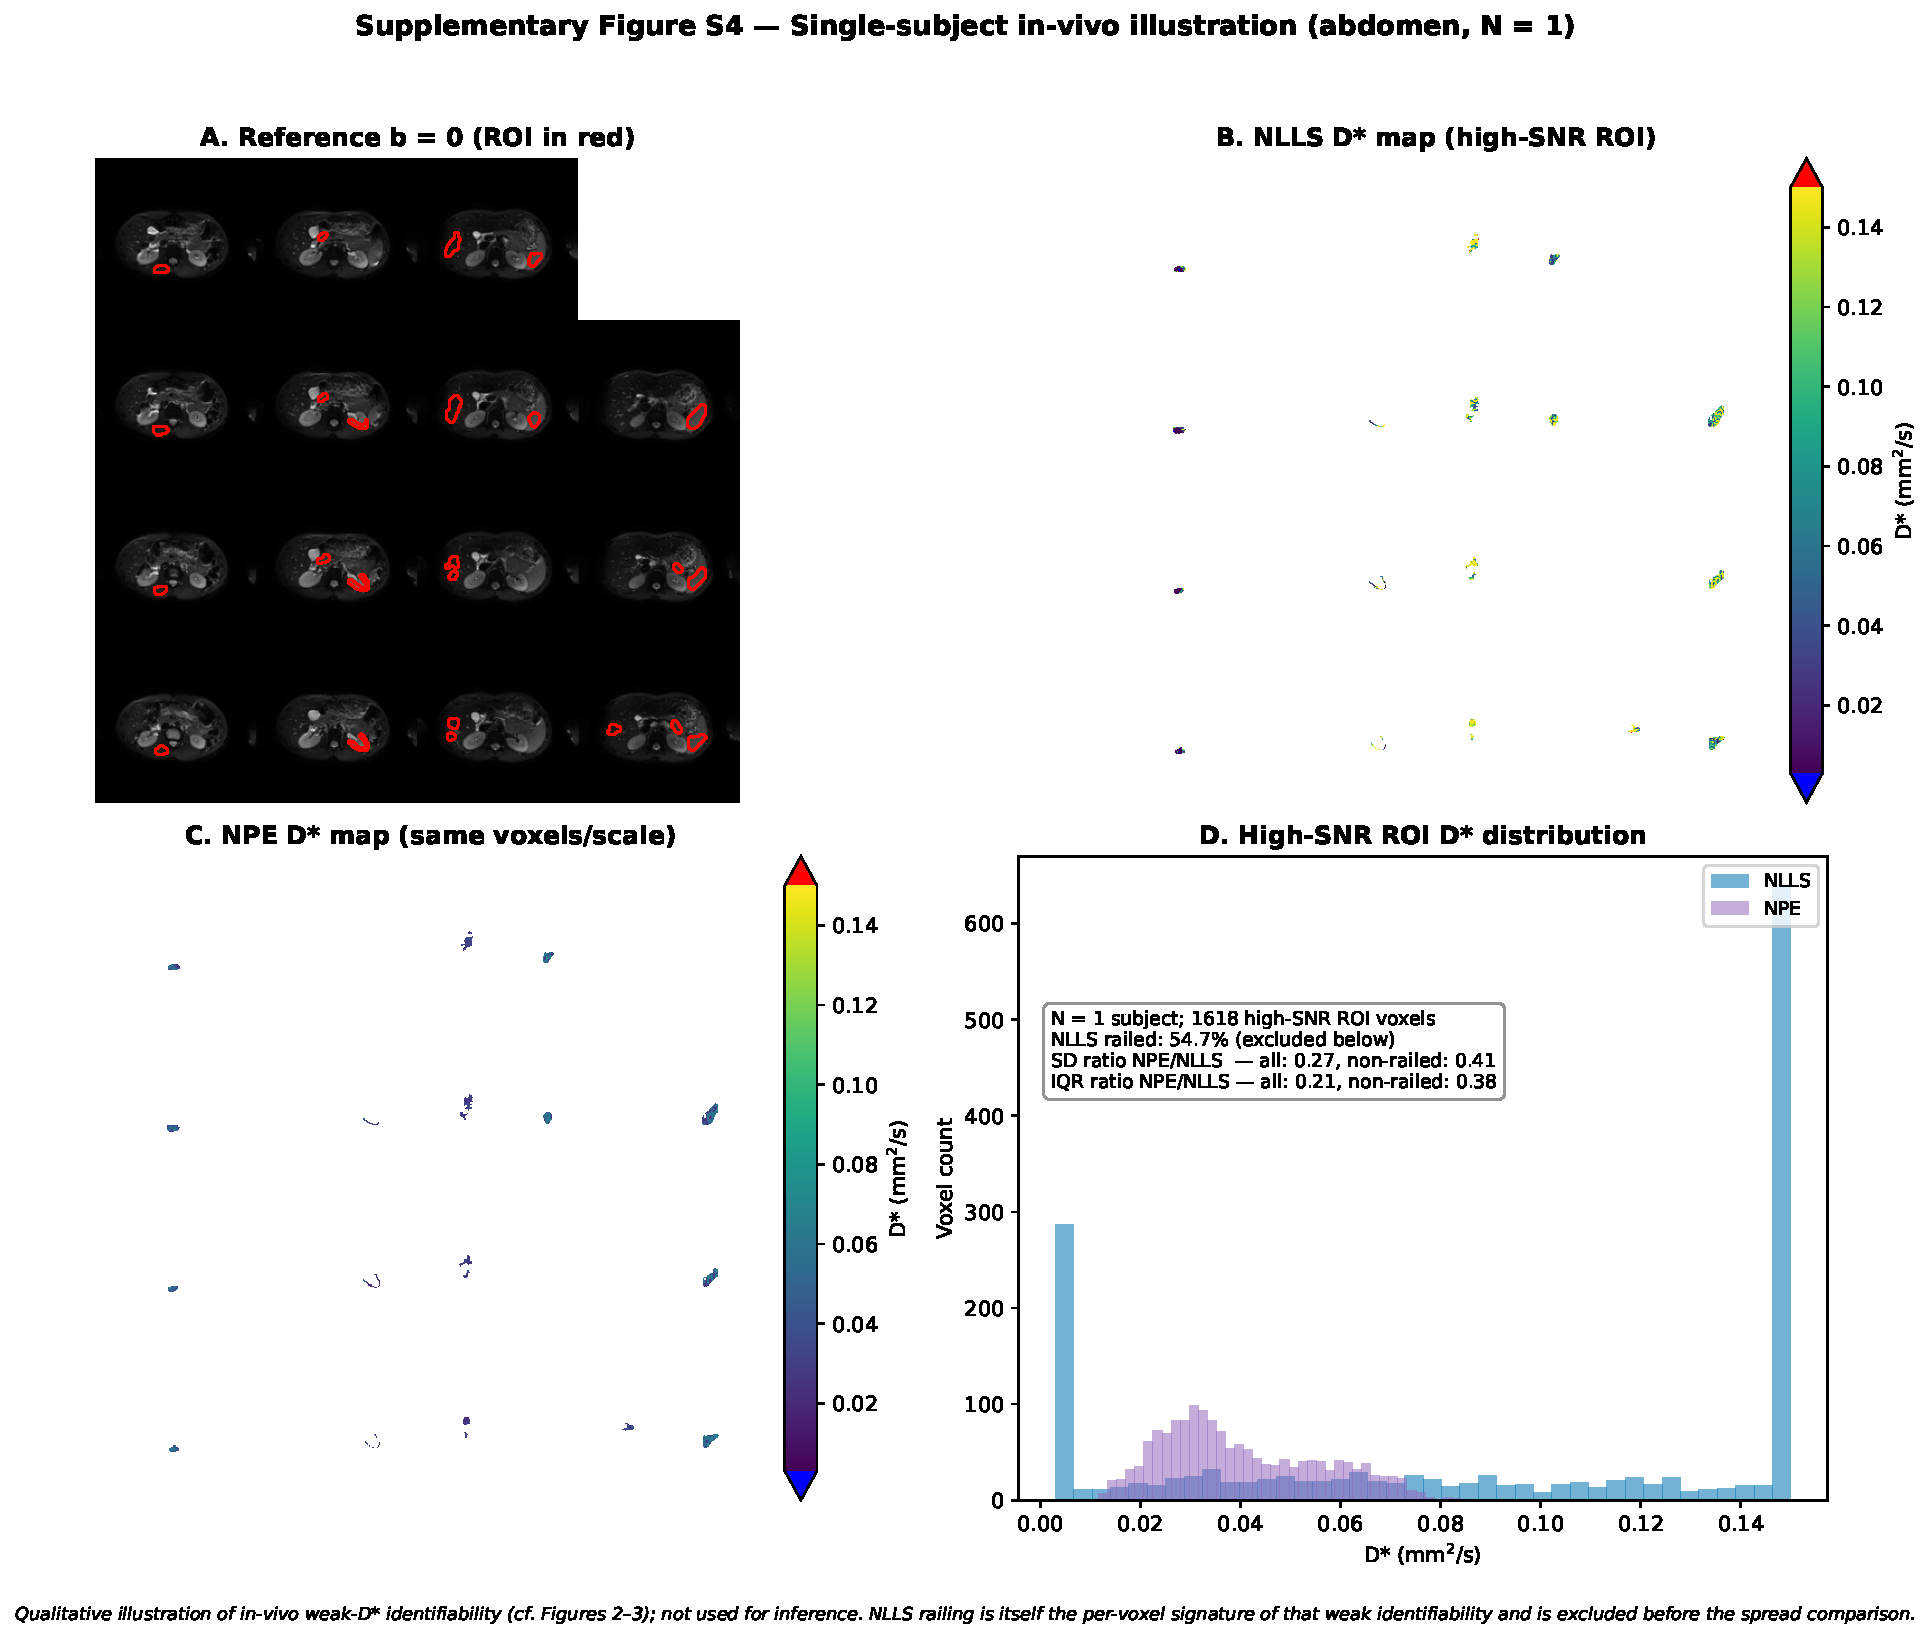
\includegraphics[width=\textwidth]{figS4_invivo_illustration.pdf}
\caption{Single-subject in-vivo illustration (abdomen, $N = 1$). NPE and biexponential-NLLS
\Dstar{} maps for one open IVIM abdominal acquisition from the same collection (OSIPI TF2.4
IVIM-MRI Code Collection data, Zenodo doi:10.5281/zenodo.14605039). In 54.7\% of high-SNR ROI
voxels the NLLS \Dstar{}
estimate is boundary-railed, which is the per-voxel signature of the weak \Dstar{}
identifiability characterised in simulation (Figures 2--3). These voxels are excluded before
the spread comparison. The case is shown as a qualitative illustration of that mechanism in
vivo and is not used to support any quantitative claim; $N = 1$ precludes population inference.}
\end{figure}

\begin{figure}[htbp]
\centering
\includegraphics[width=\textwidth]{figS5_prior_ablation.pdf}
\caption{Prior-sensitivity ablation. Fraction of \Dstar{} grid points with claimed SD below
the CRLB floor, by SNR, for the primary log-uniform prior versus a tissue-informed
truncated-Normal \Dstar{} prior (otherwise identical recipe). The below-floor overconfidence
persists, and is slightly higher, under the tissue prior at every SNR (overall 76.3\% versus
69.5\%). An informative prior legitimately permits posterior width below the prior-free CRLB,
so the discriminating evidence is the persistence under the uninformative log-uniform prior
and in both claimed and achieved SD, indicating the overconfidence is intrinsic to the
amortized estimator rather than prior-reversion.}
\end{figure}

\begin{figure}[htbp]
\centering
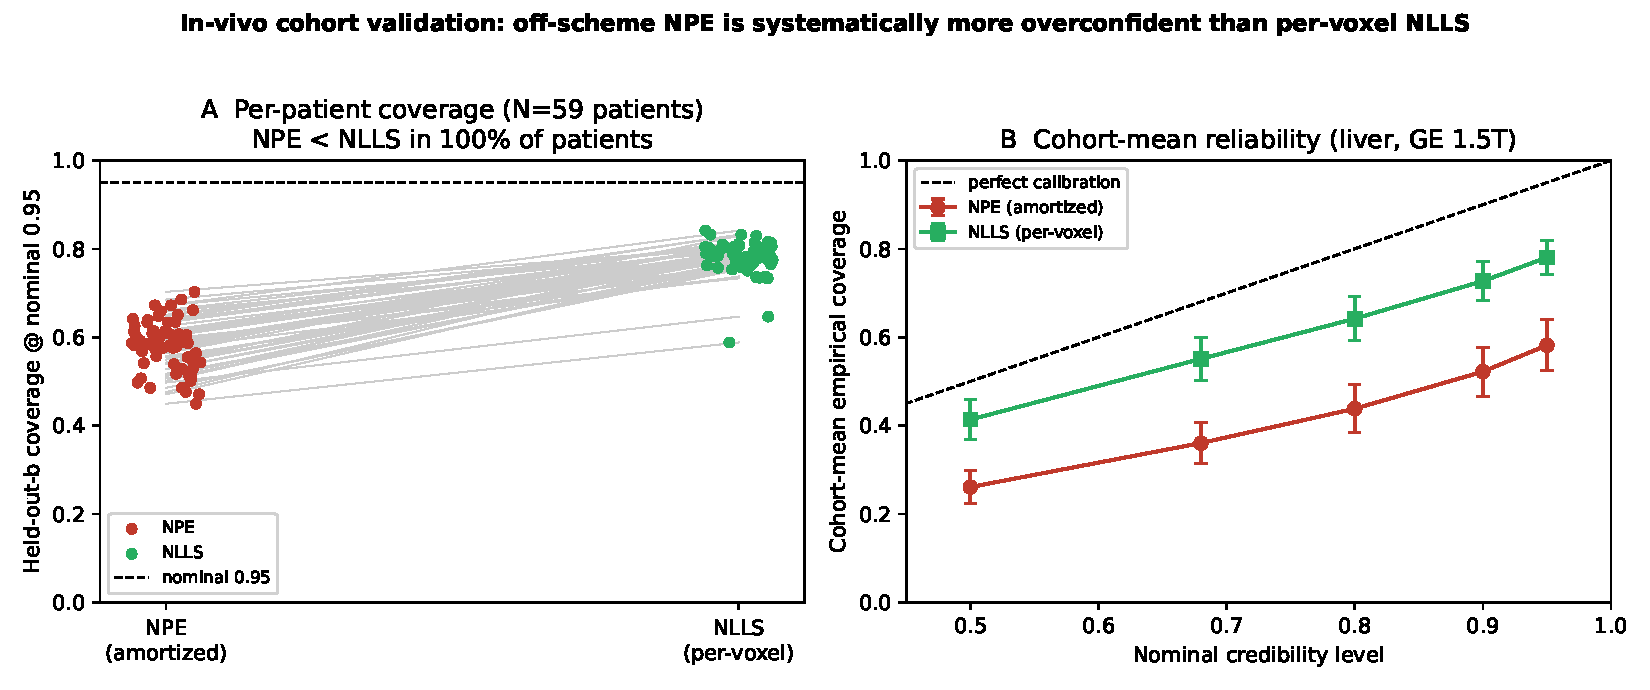
\includegraphics[width=\textwidth]{figS6_liver_cohort.pdf}
\caption{In-vivo cohort validation on an open multi-subject liver IVIM dataset ($N = 59$
patients; GE 1.5T; off-scheme for the amortized NPE). (A) Per-patient held-out-b coverage at
nominal 0.95, NPE versus the per-voxel NLLS reference (paired; each grey line is one patient).
The amortized NPE under-covers held-out signal relative to NLLS in 100\% of patients (cohort-mean
0.58 vs 0.78). (B) Cohort-mean reliability (empirical vs nominal coverage): the NPE sits below
NLLS at every credibility level. In vivo lacks voxel-level ground truth, so this compares the
two estimators rather than either against truth; NLLS is itself below nominal (model misfit and
inter-series noise), but the systematic NPE-below-NLLS gap across an independent vendor, organ,
and b-scheme shows the amortized overconfidence under acquisition shift is reproducible at cohort
scale, not a single-dataset artifact.}
\end{figure}

\end{document}
